\section{System Architecture}
We address the following problem: given a multilingual news article, assign multiple labels from a two-level taxonomy of narratives and subnarratives.

A promising recent approach to HMLC, which we refer to as H3Prompting, was introduced by \citet{singh-etal-2025-gatenlp}. 
This method decomposes the hierarchical classification task into a sequence of zero-shot LLM queries, where an initial prompt determines the top-level category, and subsequent prompts classify second-level narratives conditioned on the first-level prediction. 
In the spirit of reproducible research, we first aimed to replicate this method. 
However, the lack of publicly available implementation details prevented a direct reproduction, motivating our development of an open and configurable framework to systematically investigate zero-shot HMLC strategies.

Our investigation into a robust zero-shot HMLC framework followed an iterative design process. 
%We began by analyzing a promising top-down prompting approach, then developed 
First, we propose a traceable self-refining pipeline. Second, upon identifying its limitations, we present our more robust multi-agent ensemble approach.

%\subsection{Baseline Inspiration: Top-Down Zero-Shot Classification}



\subsection{Traceable Actor-Critic Pipeline}

Our \textbf{Actor-Critic Pipeline} aims to improve the reliability and transparency of a single agent's output. 
In zero-shot classification context, simple label outputs lack traceability and auditability, and are susceptible to unverified hallucinations. To overcome this, we propose a multi-stage pipeline reframing the task from simple classification to evidence-grounded claim generation and validation.

<<<<<<< HEAD
Our implementation uses the LangGraph framework to structure the process as a cyclical state graph \citep{langgraph2024}. The pipeline configuration is managed by a \texttt{ConfigurableGraphBuilder}, allowing components like validation to be enabled or disabled and different LLMs to be assigned to specific nodes via a YAML file. For the Actor-Critic experiments, we use Gemini 2.5 Flash as the underlying LLM for both the Actor and Critic agents. The workflow proceeds through several stages, as illustrated in Figure~\ref{fig:actor_critic_pipeline}.

\begin{figure}[!ht]
\centering
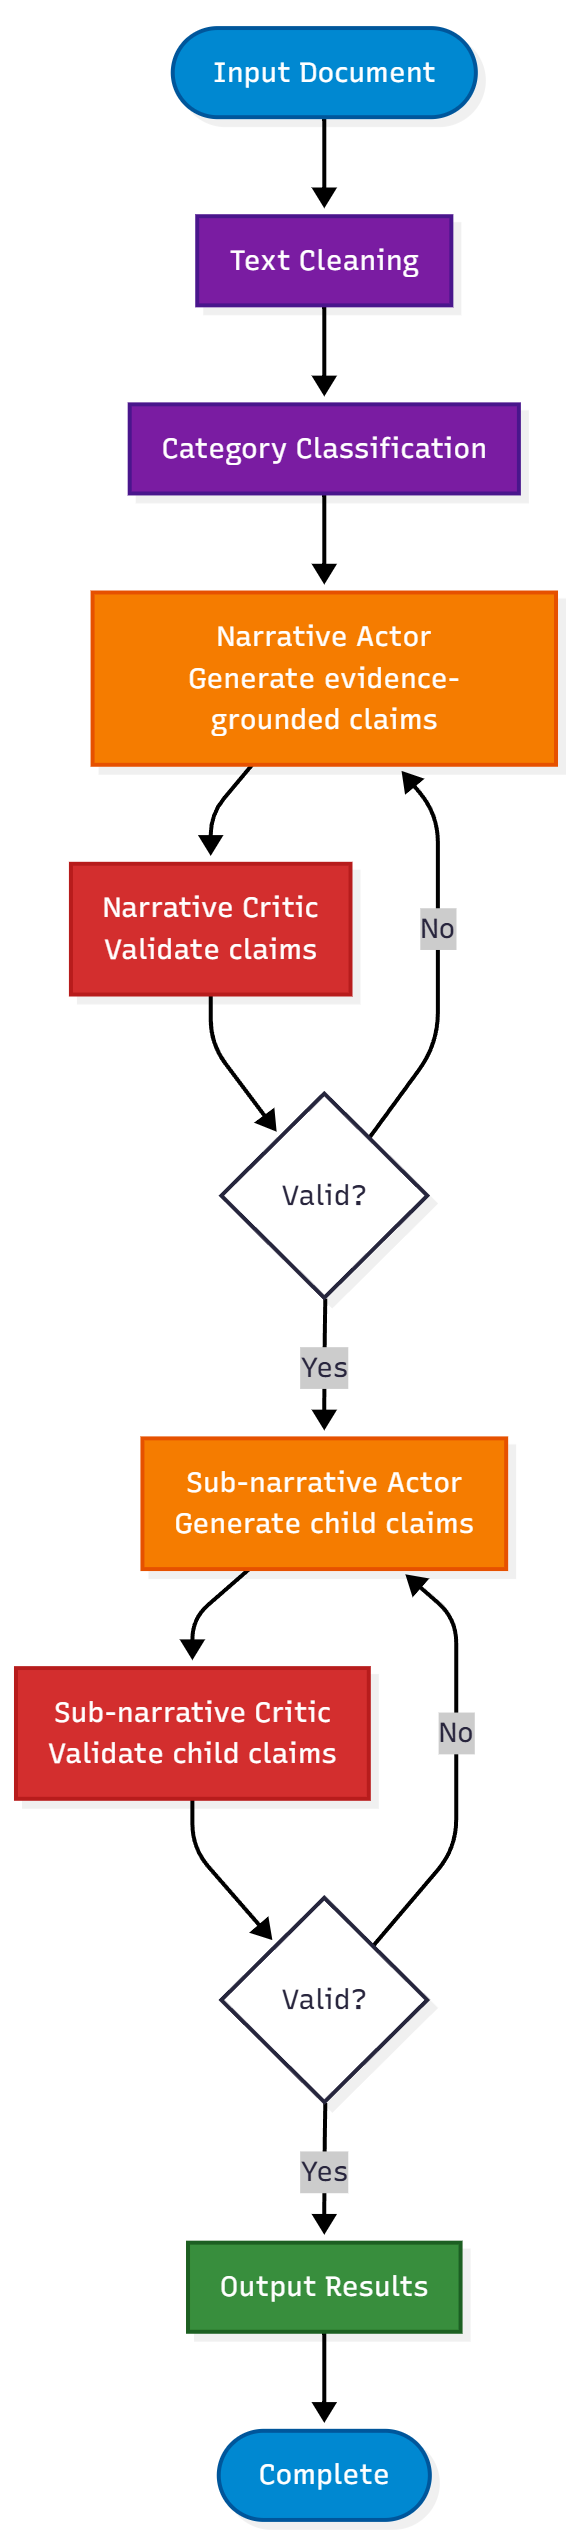
\includegraphics[height=17cm]{assets/diagrams/actor-critique.png}
\caption{Actor-Critic pipeline architecture. HMLC task is decomposed into hierarchical stages where a Narrative Actor generates evidence-grounded claims, which are then validated by a Narrative Critic. Feedback loops enable iterative refinement before getting to sub-narrative classification.}
\label{fig:actor_critic_pipeline}
\end{figure}
=======
Our implementation uses the LangGraph framework to structure the process as a cyclical state graph \citep{langgraph2024}. The pipeline configuration is managed by a \texttt{ConfigurableGraphBuilder}, allowing components like validation to be enabled or disabled and different LLMs to be assigned to specific nodes via a YAML file. For the Actor-Critic experiments, we use Gemini 2.5 Flash as the underlying LLM for both the Actor and Critic agents. The workflow proceeds through several stages (detailed below and visualized in Appendix Figure~\ref{fig:actor_critic_pipeline}).
>>>>>>> 86e8792dff0f763fe7ff81ceed3a56b3a6ba8d62

\textbf{Category Classification.} 
An initial node determines the document's domain (e.g. Climate Change (CC) or Ukraine-Russia-War (URW)) to focus subsequent stages on the relevant subset of the narrative taxonomy.

\textbf{The Narrative Actor (Claim Generation).}
The ``Actor'' is an LLM agent prompted to act as an expert analyst. For each narrative it identifies, it must generate a structured JSON object containing the \texttt{narrative\_name}, a verbatim \texttt{evidence\_quote} from the text, and reasoning that connects the two.

\textbf{The Narrative Critic (Claim Validation).}
The Actor's output is passed to the ``Critic,'' a separate LLM agent with a distinct, skeptical persona. The Critic validates the Actor's claims against strict criteria (evidence accuracy, relevance, completeness). If the Critic finds flaws, it generates structured feedback, and the graph's conditional logic routes the state back to the Actor for a retry, incorporating the feedback into a refinement prompt.

\textbf{Sub-narrative Actor and Critic.}
Once narratives are set, the process repeats hierarchically. A Sub-narrative Actor generates claims for each parent narrative, which are then validated by a Sub-narrative Critic, also with a self-correction loop.

%\vspace{0.5cm}
This evidence-grounded architecture offers significant advantages in traceability and auditability, as every prediction is grounded in a textual \texttt{evidence\_quote}, a process we enhanced using LangSmith for detailed debugging and prompt refinement \citep{langsmith2024}. However, while this pipeline showed promise, our experiments revealed that it introduced its own form of instability. The process was highly sensitive to the quality of the Critic's feedback, which, being LLM-generated, was itself prone to stochasticity. A flawed critique could send the Actor down an unproductive refinement path, sometimes degrading performance. This reliance on a single, fallible ``critic'' highlighted a fundamental bottleneck and motivated our shift towards a more robust consensus mechanism.

\subsection{Prompt Engineering Strategy}

A critical component of both the Actor-Critic and Agora frameworks is the systematic design of prompts that guide the LLM's classification behavior. Our prompting strategy incorporates several key principles:

\noindent\textbf{1. Structured Output Format.} 
All classification prompts enforce structured JSON output with required fields (\texttt{narrative\_name}, \texttt{evidence\_quote}, and \texttt{reasoning}). 
This ensures that every classification decision is explicitly grounded in textual evidence, enabling traceability and facilitating automated validation. For example, the narrative classification prompt specifies:

\begin{quote}
\small
\textit{``Your entire response MUST be a single JSON object. ALL fields in the schema below are REQUIRED. Do not omit any fields.''}
\end{quote}

\noindent This strict formatting requirement forces the model to provide explicit justifications, preventing opaque label predictions.

\noindent\textbf{2. Chain-of-Thought Reasoning.} 
Prompts explicitly instruct the model to perform step-by-step internal reasoning before producing the final classification. 
This approach, inspired by chain-of-thought prompting \citep{wei2022chain}, encourages the model to identify key phrases, evaluate each potential label \textit{vs.} the evidence, and formulate explicit justifications. 
The narrative classification prompt includes:

\begin{quote}
\small
\textit{``Step 1: Chain of Thought (Internal Reasoning). First, think step-by-step to analyze the provided text. Identify key phrases, arguments, and themes. For each potential narrative from the list, consider if it applies. Find a specific, direct quote from the text that serves as the strongest evidence for each narrative you believe is present.''}
\end{quote}

\noindent This two-step process (reasoning, then formatting) reduces impulsive classifications and improves output quality.

\noindent\textbf{3. Hierarchical Prompt Design} 
The classification process uses distinct prompts at each level of the hierarchy:
\begin{itemize}
\item \textbf{Category Classification}: A strict topical classifier that determines text domain (e.g. Climate Change (CC) or the Ukraine-Russia War (URW)). 
The prompt enforces strict labeling: 
\begin{quote}
\small
\textit{``Output EXACTLY one label token enclosed in square brackets on the next line: [URW], [CC], or [Other].''}
\end{quote}

\item \textbf{Narrative Classification}: Given the domain, the model selects from domain-specific narratives, with each narrative accompanied by its definition, examples, and classification instructions according to the template:
\begin{quote}
\small
\textit{``- \{Category\}: \{Narrative Name\}\\
\hspace*{1em}Definition: \{Definition text\}\\
\hspace*{1em}Example: \{Example text\}\\
\hspace*{1em}Instruction: \{Instruction text\}''}
\end{quote}

\item \textbf{Sub-narrative Classification}: Given a parent narrative, the model identifies more fine-grained sub-narratives, including an ``Other'' option for cases where the text supports the parent narrative but does not fit specific sub-narrative definitions. The prompt explicitly instructs: 
\begin{quote}
\small
\textit{``Step 2: Check for a Remainder. Are there any other phrases or arguments that support the parent narrative but were NOT used as evidence for the specific subnarratives? Step 3: Add `Other' if Necessary.''}
\end{quote}
\end{itemize}

\noindent\textbf{4. Critic Prompts and Refinement.} 
In the Actor-Critic pipeline, the Critic agent receives a specialized prompt that adopts a ``meticulous and skeptical editor'' persona. The Critic evaluates classifications against strict criteria: evidence accuracy (verbatim quotes), relevance (direct support for the label), and completeness (no obvious narratives missed). The critic prompt states:

\begin{quote}
    \small
\textit{``You are a meticulous and skeptical editor. Your task is to evaluate a classification of propaganda narratives applied to a text. You must be extremely strict. The classification is only valid if every narrative is strongly and explicitly supported by the provided evidence from the text.''}
\end{quote}

\noindent When validation fails, a refinement prompt incorporates the Critic's feedback: 
\begin{quote}
    \small
    \textit{``You previously analyzed a text, but your analysis had flaws. A meticulous editor has provided the following feedback. Your task is to re-analyze the text, incorporating this feedback to produce a new, corrected classification.''} 
\end{quote}
    \noindent This feedback loop enables iterative self-correction.

The complete prompts used in our experiments are provided in Appendix~\ref{appendix:prompts}.

\subsection{Proposed Framework: Agora Multi-Agent Ensemble}

To overcome the limitations of a single-critic system and the broader issue of single-agent stochasticity, we developed Agora, a multi-agent ensemble framework. The core principle of Agora is to replace the judgment of a single agent (or a single critic) with the collective ``wisdom of the crowd,'' leveraging the consensus of multiple independent agents to arrive at a more stable and accurate classification.

Importantly, Agora uses the same core prompts as the baseline and Actor-Critic systems (without the Critic validation step). This design choice isolates the effect of the ensemble mechanism itself, allowing us to attribute performance improvements specifically to the consensus-based aggregation rather than to prompt engineering differences. For the Agora experiments, we use GPT-5-nano as the underlying LLM for all agents in the ensemble, with $N=3$ agents by default.

The framework operates via a fan-out, fan-in process for each level of the hierarchy (e.g., Narrative classification).

\paragraph{Fan-Out (Parallel Classification).} 
Instead of a single LLM call, Agora instantiates $N$ independent agents (where $N$ is a configurable parameter). The same input text and prompt are sent to all $N$ agents, who perform the classification in parallel. This step effectively samples $N$ independent points from the LLM's output distribution for the given task.

\paragraph{Fan-In (Aggregation via Voting).} 
After all $N$ agents return their individual classifications, an Aggregation node consolidates the results using a voting scheme. We implemented and evaluated three distinct aggregation strategies:

\begin{itemize}
\item \textbf{Union:} The final label set includes any label proposed by at least one agent. This high-recall strategy is useful for identifying all potential labels.

\item \textbf{Intersection:} The final label set includes only those labels that all agents unanimously agreed upon. This high-precision strategy filters out all but the most confident predictions.

\item \textbf{Majority Vote:} The final label set includes any label proposed by more than half ($> N/2$) of the agents. This strategy provides a robust balance between precision and recall, filtering out stochastic, outlier classifications while retaining a strong consensus.
\end{itemize}

\begin{figure*}[!ht]
\centering
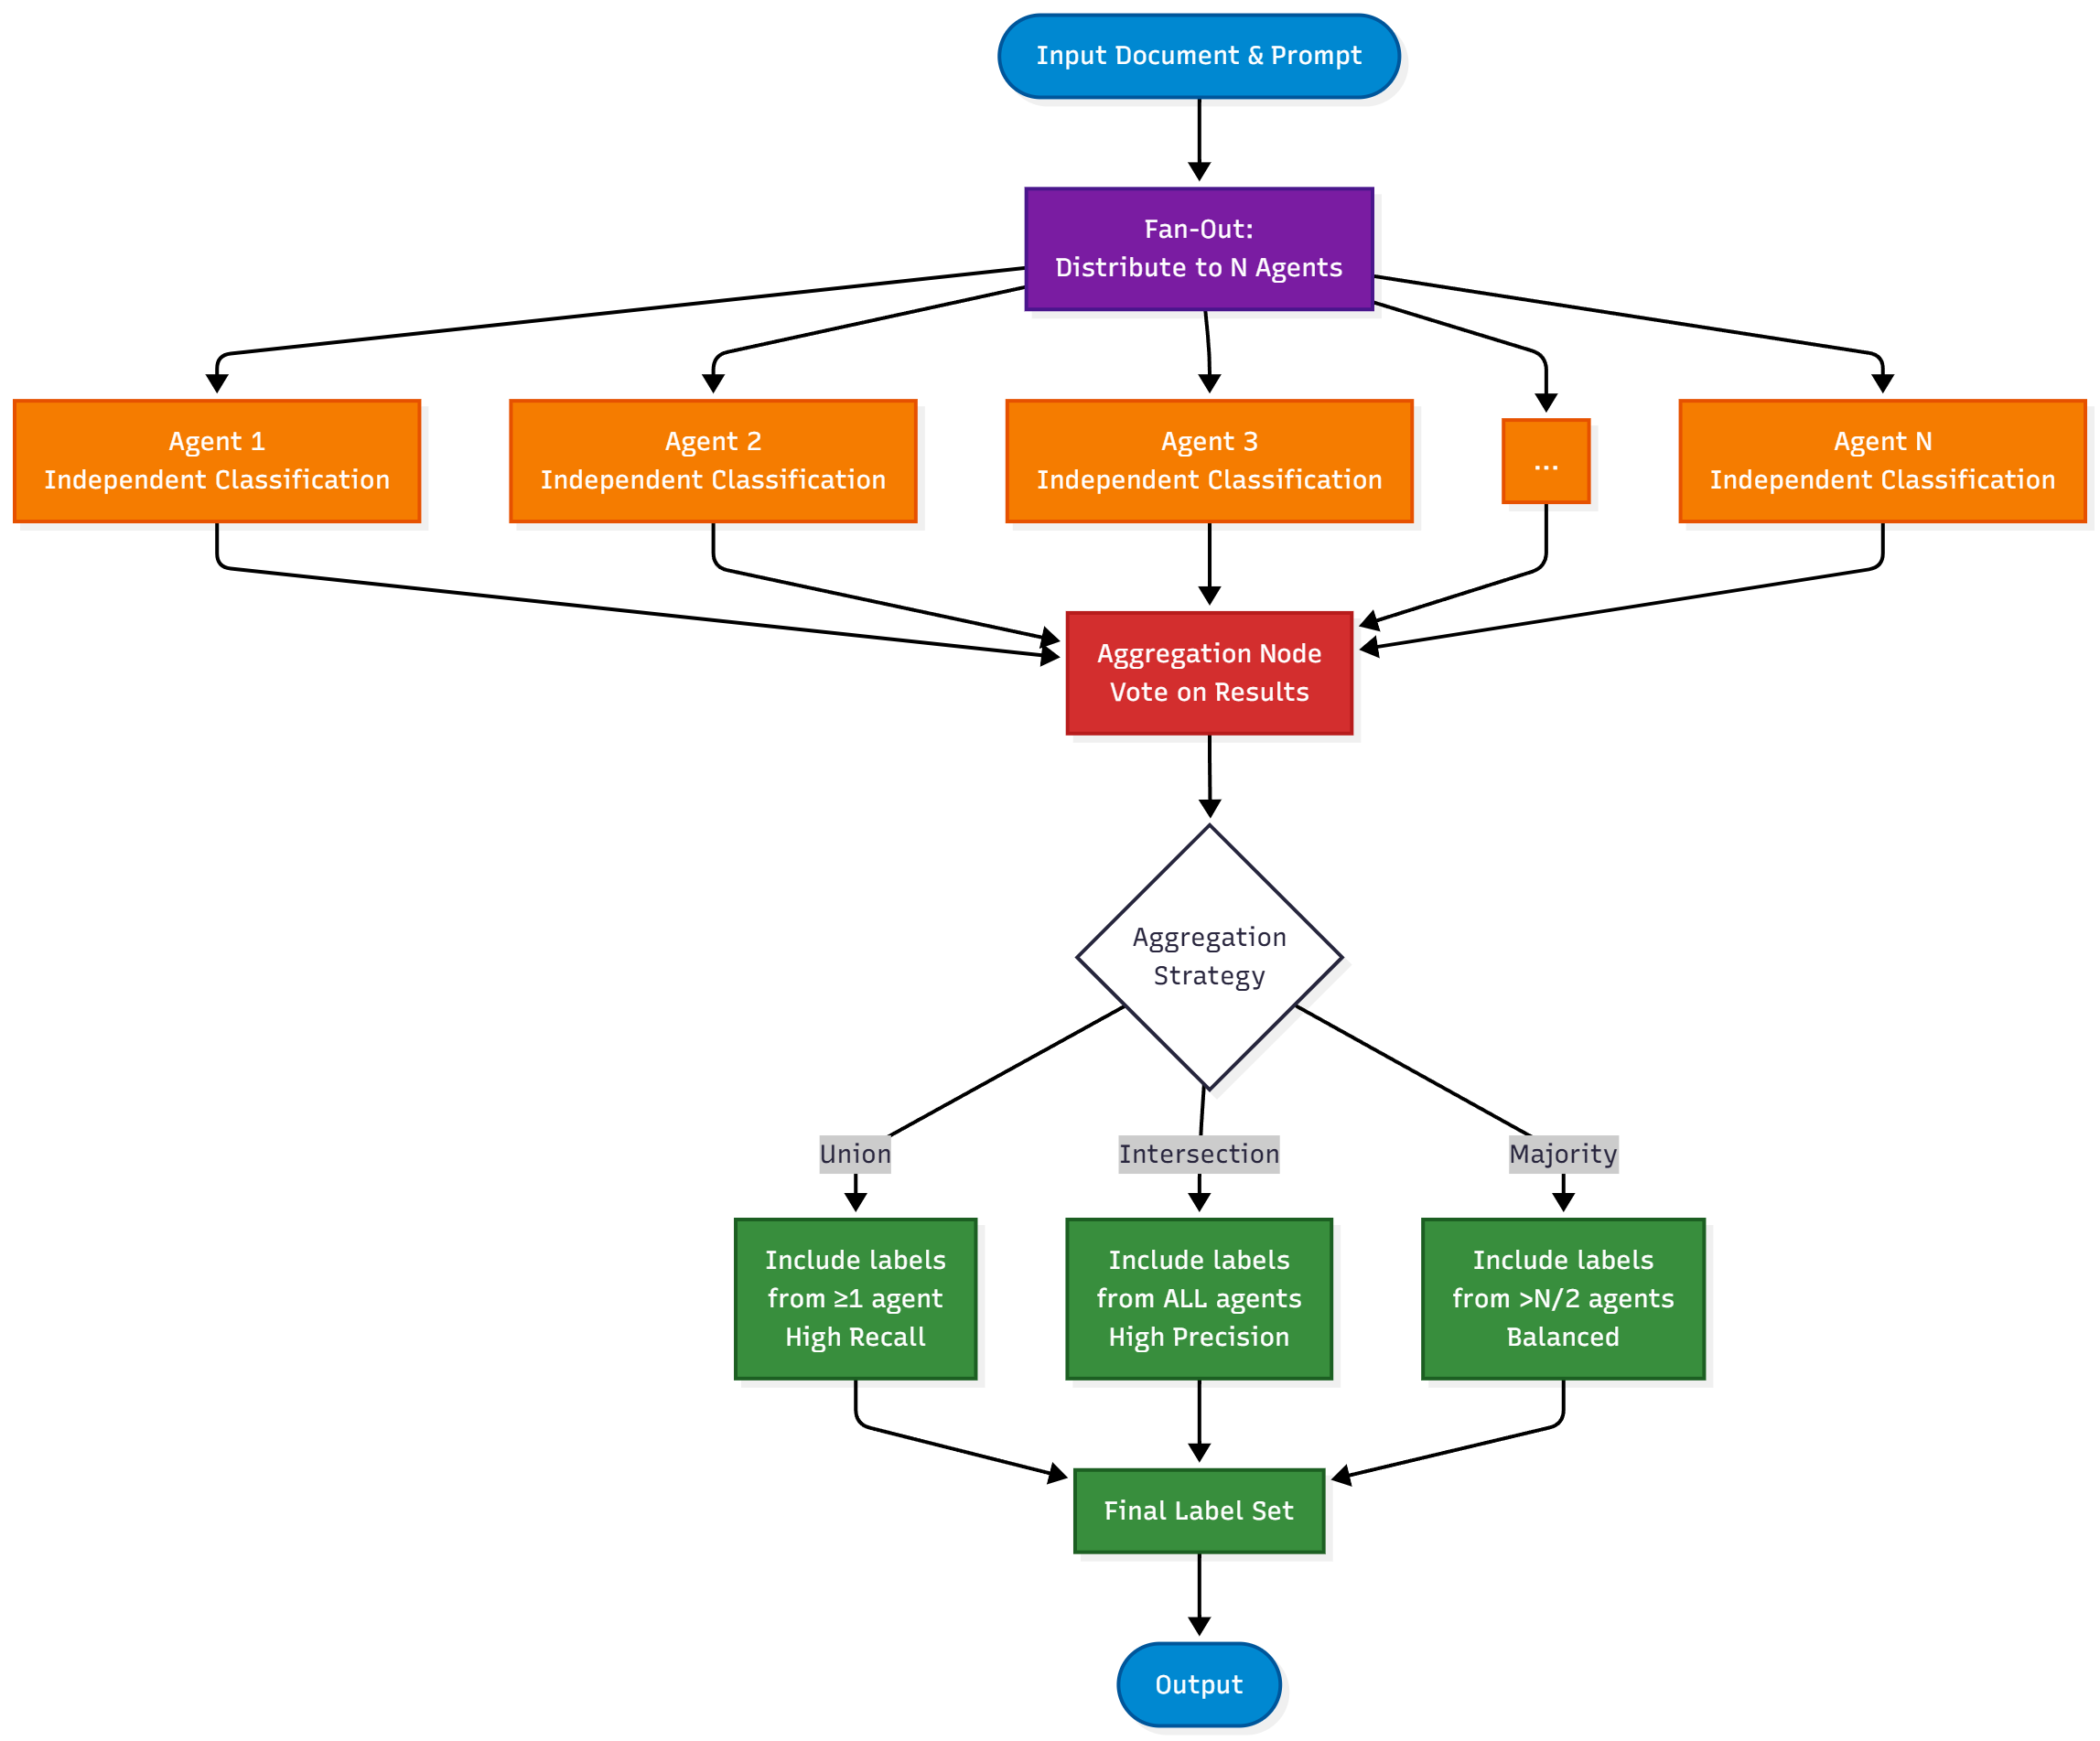
\includegraphics[height=11cm]{assets/diagrams/vote-based.png}
\caption{Agora multi-agent ensemble architecture. The classification task is distributed to $N$ independent agents in parallel (Fan-Out), aggregates their results using a voting mechanism (Fan-In), and produces a final label set based on the chosen aggregation strategy (Union, Intersection, or Majority Vote).}
\label{fig:vote_based_ensemble}
\end{figure*}

This ensemble approach directly addresses the single-point-of-failure issue observed in the Actor-Critic pipeline. Instead of relying on one critic's potentially noisy feedback, Agora relies on the statistical robustness of a majority decision, providing a more reliable and conceptually simpler method for improving classification quality.
